\chapter{Testy systemu}
W tym rozdziale przedstawione są różne konfiguracje pakietów, wraz z wykresami ruchów platform, oraz wnioski płynące z tych zachowań.
Każdy test wymaga innego podłączenia komponentów do siebie nawzajem.

Wyniki pomiarów zostały zebrane za pomocą ROSowego narzędzia \texttt{rosbag}, a następnie wyeksportowane do pliku CSV. Za pomocą programu Gnuplot narysowano wykresy.

\section{Porównanie modeli dynamiki i kinematyki}
	Posiadając model kinematyczny, którego ruch jest sterowany wzorami, można porównać jego pozycję i rotację z modelem dynamicznym.
	Należy w tym samym momencie nadać bazom identyczne prędkości kół i zebrać dane dotyczące wzajemnej pozycji.
	Modele rozpoczynają jazdę z punktu (0,0), początkowo stoją 5 s w miejscu, aż symulator i wszystkie komponenty się załączą.
	
	Te eksperymenty pozwalają sprawdzić, jak model dynamiczny zachowuje się w stosunku do idealnego modelu kinematycznego.
	
	\begin{figure}[H]
		\centering
		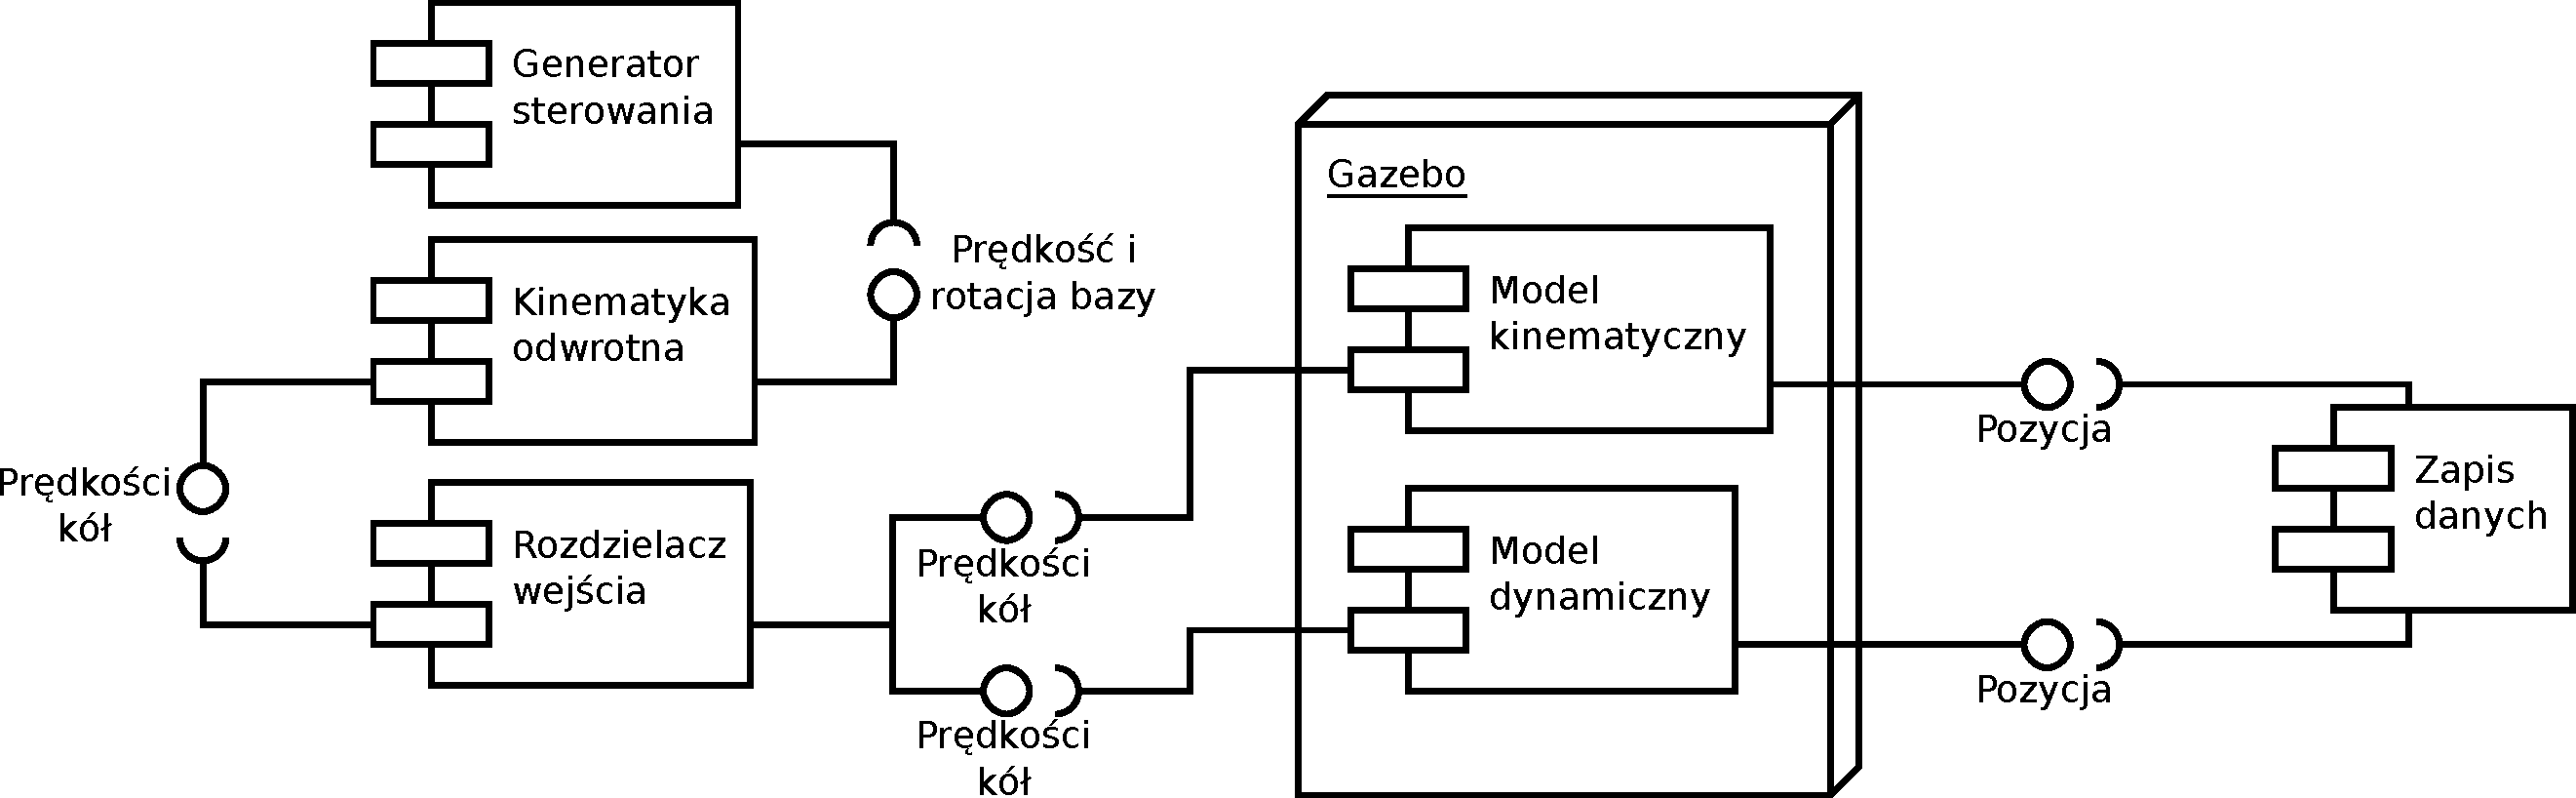
\includegraphics[width=\textwidth]{uml/gramofon.pdf}
			\caption{Połączenie komponentów w celu przetestowania wzajemnego ruchu modelu kinematycznego i dynamicznego.}
		\label{uml:gramofon}
	\end{figure}
	
	\subsection{Ruch po kwadracie}
		Wywołano ruch z prędkością 0,2 $\frac{m}{s}$ po kwadracie o boku 1 m, bez nadawania prędkości kątowej.
		Modele przejechały ścieżkę pięciokrotnie, po czym zatrzymały się. W kątach kwadratu nie było nadania prędkości zerowej.
		
		Celem tego eksperymentu było sprawdzenie, czy model dynamiczny będzie wykazywał odchylenia w trakcie jazdy po prostej ścieżce 
		i jak będzie reagował na nagłe zmiany kierunku jazdy.
		
		\begin{figure}[H]
			\centering
			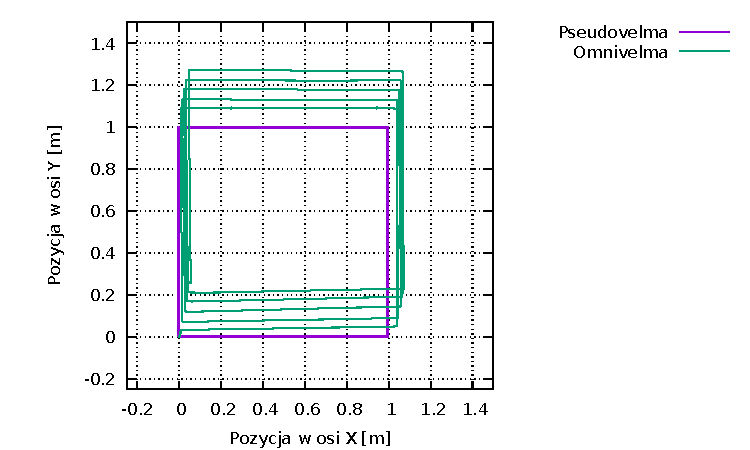
\includegraphics[width=\textwidth]{plots/square.pdf}
				\caption{Ruch modelu kinematycznego i dynamicznego po kwadratowej ścieżce.}
			\label{plot:gramofon_square}
		\end{figure}
		
		Po pierwsze widać, że tuż przed rozpoczęciem jazdy model dynamiczny odsunął się o kilka centymetrów od pozycji początkowej i obrócił nieznacznie.
		Jest to spowodowane tym, że maszyna do symulacji fizyki działa na liczbach zmiennoprzecinkowych pojedynczej precyzji,
		zatem nie wszystkie siły działające na obiekty będą się dokładnie równoważyć i może istnieć mały ruch w losowych kierunkach i rotacja.
		
		Następnie, po nadaniu ruchu w bok, platformy jechały po linii prostej.
		Model dynamiczny wykonał większą trasę do modelu kinematycznego, co nie jest spowodowane poślizgiem.
		Na takie zachowanie wpływa wiele czynników, zarówno wewnętrzna implementacja maszyny symulacyjnej fizyki, jak i natura użytych algorytmów.
		
		Przy zmianie prędkości widać poślizg przy zatrzymywaniu się z danego kierunku.
		Kąty trasy są zaokrąglone w jednym kierunku, co pokazuje że model dynamiczny posiada bezwładność. 
		Gdy otrzymuje nowe prędkości kół, nadal porusza się jeszcze przez pewien czas w poprzednim kierunku.
		Poślizg przy ruszaniu jest mniejszy.
		To zjawisko nie wpływa istotnie na trasę modelu, gdyż przy testach, w których prędkość zmieniała się wolno i w których nie występowały nagłe hamowania,
		nadal występowało takie samo zboczenie w stosunku do trasy kinematycznej.
		
		Za każdym obiegiem pętli narasta różnica pozycji wynikającej z kinematyki i pozycji obliczonej przez symulator.
		Po zatrzymaniu się modelu dynamicznego, ponownie porusza się on jeszcze przez pewien czas w losowym kierunku, innym niż na początku,
		aż do przerwania testu.
	
	\subsection{Ruch po ,,rozecie''}
		Drugi, bardziej skomplikowany test składa się na ruchy platform w przód i w tył, oraz obrót wokół punktu.
		
		Modele jechały 2 m w przód z prędkością 0,25 $\frac{m}{s}$, następnie następował obrót o 45°, po czym odbywała się jazda w tył.
		Na koniec ruch w bok przy jednoczesnym obrocie i powtórzenie cyklu. Czterokrotne wykonanie tego zamyka trasę.
		
		\begin{figure}[H]
			\centering
			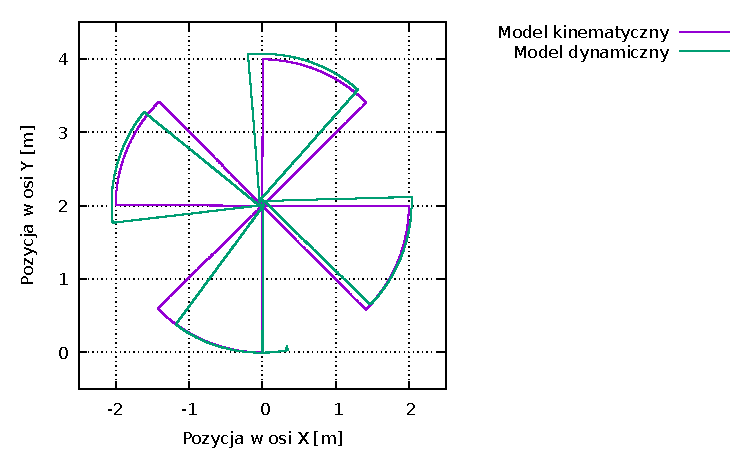
\includegraphics[width=\textwidth]{plots/sun.pdf}
				\caption{Ruch modelu kinematycznego i dynamicznego po rozetowej ścieżce.}
			\label{plot:gramofon_sun}
		\end{figure}
		
		Z wykresu wywnioskować można, prócz tego co z poprzedniego eksperymentu, to że model dynamiczny przegania model kinematyczny również w kwestii obrotu.
		W tym przypadku składowa trasy pionowej (w lokalnym układzie), czyli prędkość w przód i w tył, zniosła się.
		Obrót i ruch w bok były ciągle narastające, a co za tym idzie, spowodowały przesunięcie się modelu dynamicznego, co widać, porównując ich końcową pozycję.
		
	\subsection{Powtarzalność testów}
		Pomimo, że na środowisko wirtualne w maszynie symulacyjnej fizyki nie działają żadne zjawiska zewnętrzne, nadal jej działanie zależy od wewnętrznych niedoskonałości
		systemu, na którym działa. W to wchodzą takie rzeczy, jak niedokładności w reprezentacji liczb zmiennoprzecinkowych, czas pomiędzy kolejnymi klatkami symulacji i 
		niedeterministyczne przekazywanie wiadomości przez system operacyjny.
		
		Zatem każdy test będzie generował nieco inne wyniki pozycji modelu zarówno kinematycznego, jak i dynamicznego. 
		Jednak w kinematycznym przypadku różnice są niezauważalne.
		Przeprowadzono powyższe testy trzykrotnie, aby zbadać jak bardzo każdy z przejazdów modelu różni się od poprzedniego.
		
		\begin{figure}[H]
			\centering
			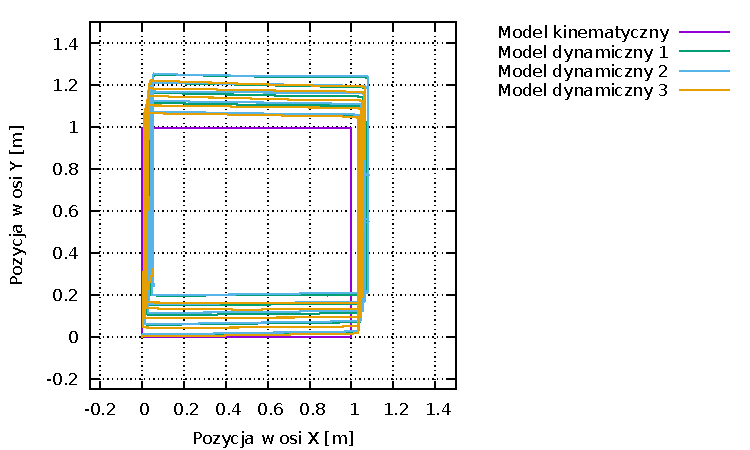
\includegraphics[width=\textwidth]{plots/square_3.pdf}
				\caption{Wielokrotny ruch modelu kinematycznego i dynamicznego po kwadratowej ścieżce.}
			\label{plot:gramofon_square_3}
		\end{figure}
		
		\begin{figure}[H]
			\centering
			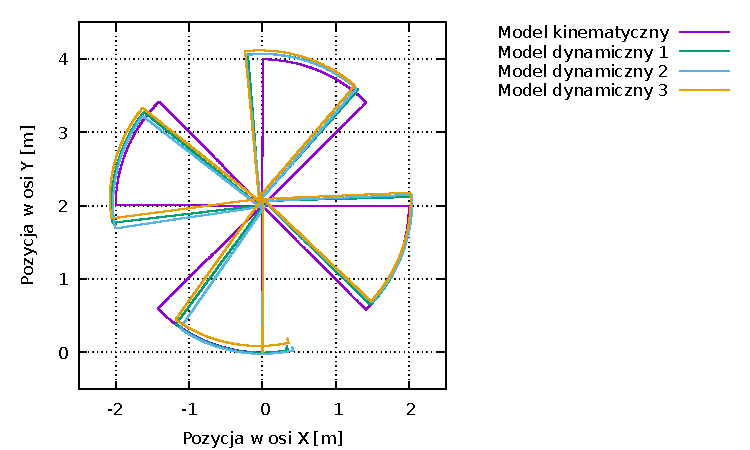
\includegraphics[width=\textwidth]{plots/sun_3.pdf}
				\caption{Wielokrotny ruch modelu kinematycznego i dynamicznego po rozetowej ścieżce.}
			\label{plot:gramofon_sun_3}
		\end{figure}
		
		Wygląda to tak, że odległość pomiędzy pozycjami modelu dynamicznego w różnych testach zwiększa się w czasie.
		Różnica narasta wraz z pokonaną odległością.
		Takie zjawisko jest typowe dla symulacji w których istnieje wiele czynników zewnętrznych, wpływających na symulację.
		
		Aby zmniejszyć te niedoskonałości, należałoby, po pierwsze uruchomić symulację na systemie czasu rzeczywistego, a po drugie zwiększyć 
		dokładność reprezentacji liczb zmiennoprzecinkowych, a co za tym idzie, znacząco zwiększyć obciążenie procesora.
		
		Nie można nadal pozwolić na to, aby symulacja przestała odbywać się w czasie rzeczywistym, gdyż to spowodowałoby opóźnienia w ruchu platform.
		Ponieważ, na przykład, jeśli program sterujący wywoła przez sekundę ruch z prędkością 1 $\frac{m}{s}$, aby przejechać dystans 1 m,
		a obciążony symulator będzie nadawał tą prędkość przez ten czas, to w stosunku od obciążenia, może być to inny czas symulacji.
		Zatem patrząc z perspektywy modelu, sterowanie platformie nadawane będzie przez krótszy czas, niż zakłada to program sterujący i model przejedzie mniejszą odległość.
		Należałoby buforować wszystkie otrzymywane wiadomości i stosować je dopiero w czasie symulacji zgodnym z czasem odebrania pakietu. 
		Ale tutaj także jest problem z generowaniem danych, nawet jeśli wygenerowane dane opatrzone będą nagłówkiem z czasem symulatora, to i tak program obierający będzie miał
		problem z zastosowaniem ich. Dochodzi do problemu synchronizacji programu sterującego i symulatora w niestałym czasie. 
		Wymagałoby to stosowania marszczenia czasu i podobnych technik.
